\documentclass[conference]{IEEEtran}
\IEEEoverridecommandlockouts
% Template version as of 6/27/2024
\usepackage{cite}
\usepackage{amsmath,amssymb,amsfonts}
\usepackage{algorithmic}
\usepackage{graphicx}
\usepackage{textcomp}
\usepackage{xcolor}
\def\BibTeX{{\rm B\kern-.05em{\sc i\kern-.025em b}\kern-.08em
    T\kern-.1667em\lower.7ex\hbox{E}\kern-.125emX}}
\begin{document}

\title{FRESCA-Net: A Compact From-Scratch Convolutional Network with Energy-Domain Between-Class Learning for Environmental Sound Classification}

\author{\IEEEauthorblockN{Budi Juarto}
\IEEEauthorblockA{\textit{Bina Nusantara University} \\
Jakarta, Indonesia \\
budi.juarto@binus.ac.id}
\and
\IEEEauthorblockN{Mochamad Haldi Widianto}
\IEEEauthorblockA{\textit{Bina Nusantara University} \\
Jakarta, Indonesia \\
mochamad.widianto@binus.ac.id}
}

\maketitle

\begin{abstract}
Environmental sound classification underpins acoustic monitoring, surveillance and bioacoustic sensing, yet the field-standard ESC-50 benchmark remains hard because it offers only two thousand clips across fifty classes. Leaderboard progress is dominated by transformers pretrained on external corpora, which reach ninety-five to ninety-eight percent but are unusable when no external data, no pretraining and a small on-device budget are the operating constraints. This work proposes FRESCA-Net, a compact 2.88 M-parameter residual network trained entirely from scratch, and benchmarks it against the published from-scratch family under one leakage-free protocol. It couples a squeeze-and-excitation residual backbone with a frequency-coordinate channel, anisotropic downsampling that keeps a genuine temporal sequence, and an attentive-statistics pooling head; its main data lever is an energy-domain Between-Class mixing applied to the raw waveform before the mel transform, so the mixing stays energy-additive. Under the official five-fold cross-validation with a fixed budget, stochastic weight averaging and no checkpoint selection on the test fold, a single model reaches 81.55 percent and a three-seed ensemble 82.45 percent, exceeding human accuracy (81.3) and matching EnvNet-v2 with Between-Class learning (81.8). A matched ablation attributes 16.45 points to the architecture and 2.90 to the augmentation. Re-run without re-tuning on UrbanSound8K it reaches 74.57 percent --- clear of the classic from-scratch baselines but short of the augmented ones, so the architecture transfers while its ESC-50 ranking does not. We further profile the deployed cost --- 2.23 GMAC, 11.0 MB of weights and 100.1 ms per crop on one CPU core --- and show that multiply--accumulate counts and measured latency rank compact audio models differently, so neither alone substantiates an efficiency claim. Code, seeds and per-fold results are released.
\end{abstract}

\begin{IEEEkeywords}
environmental sound classification; ESC-50; convolutional neural networks; between-class learning; squeeze-and-excitation; attentive pooling; from-scratch training; edge audio
\end{IEEEkeywords}

\section{Introduction}
Automatically naming the sounds around us --- a dog barking, a chainsaw, rain, a crying baby --- underpins acoustic surveillance, urban noise monitoring, smart-home context sensing and bioacoustic ecology, yet a human annotator quickly becomes the bottleneck on any continuous stream of audio. The ESC-50 dataset \cite{piczak_dataset} is the reference benchmark: fifty everyday sound categories, forty clips each, in five predefined folds. Its very compactness is what makes it hard. With only two thousand five-second clips over fifty classes, a model sees roughly sixteen hundred training clips per fold and is exposed to overfitting in a way that large speech and music corpora are not; the hand-crafted baselines that accompanied the dataset reached only 44.3, 39.6 and 32.2 percent \cite{piczak_dataset}.

Convolutional networks quickly became the workhorse of the benchmark. A shallow two-convolution network on mel-spectrograms with a tall vertical first-layer filter reached 64.5 percent \cite{piczak_cnn}, and a deeper network paired with audio-specific augmentation such as time-stretching and pitch-shifting pushed it further \cite{salamon_bello}. A second line moved the input closer to the signal, learning from the raw waveform end-to-end \cite{tokozume_envnet} and with very deep one-dimensional stacks \cite{dai_rawwaveform}, while a parallel strand asked how much the time--frequency representation itself matters \cite{huzaifah_tf}. Because labelled data is so scarce, regularisation and augmentation carry an unusually large share of the accuracy: Between-Class learning, which mixes two examples in a proportion and asks the network to predict the ratio, is a particularly strong lever on environmental audio \cite{tokozume_bc}, multi-scale convolutions fusing waveform and spectrogram views add complementary gains \cite{zhu_multiscale}, and representations learned from the audio track of unlabelled video help the smallest supervised sets \cite{aytar_soundnet}.

The highest numbers on ESC-50, however, come from a different regime. Backbones trained on the AudioSet corpus of over two million weakly labelled clips \cite{hershey_cnnaudio}, \cite{gemmeke_audioset} and their descendants --- pretrained audio neural networks \cite{kong_panns}, the audio spectrogram transformer \cite{gong_ast}, a self-supervised acoustic tokeniser \cite{chen_beats} and a language--audio contrastive model \cite{elizalde_clap} --- now report ninety-five to ninety-eight percent, but they carry hundreds of hours of external supervision into a task whose own training set is two thousand clips; the same caveat applies to borrowing an ImageNet-pretrained backbone for spectrograms \cite{guzhov_esresnet}. Once external data, pretraining and the parameter and latency budget of an edge device are all removed, the honest question is how far a compact network trained from scratch can go --- and there the published numbers are both lower and scattered across protocols that do not agree on how the held-out fold is used \cite{palanisamy_rethinking}.

This study addresses that gap. We propose FRESCA-Net, a compact residual network of 2.88 million parameters trained end-to-end on ESC-50 with no external data and no pretraining, and evaluate it against the published from-scratch family under a single, deliberately leakage-free five-fold protocol: rather than selecting the best epoch on the very fold being tested --- a subtle but common source of optimism --- we fix the training budget in advance and report a stochastic-weight-averaged model, so every clip is scored once by a model that never saw its fold. On top of the architecture we run a matched two-by-two ablation that separates the contribution of the network from that of the augmentation, and a small multi-seed ensemble to probe the ceiling of the regime. The contribution is fourfold: a compact architecture that reaches human-level accuracy on ESC-50 from scratch; a clean protocol and ablation that decompose architecture from augmentation; a measured account of the inference cost --- arithmetic, memory and latency --- that a parameter count cannot supply; and a check that the recipe transfers unchanged to UrbanSound8K, with a released implementation so each can be reproduced.

\section{Materials and Methods}

\subsection{Datasets and Evaluation Protocol}
We use the ESC-50 dataset \cite{piczak_dataset} exactly as published: 2000 single-channel clips of five seconds sampled at 44.1 kHz, fifty balanced classes of forty clips, and the five author-defined folds. All experiments follow the official five-fold cross-validation --- for a held-out fold $k$ the model is trained on the other four folds and tested on $k$ --- so that each clip is tested exactly once and the mean over the five folds is a leave-one-fold-out estimate over the whole dataset. Because the classes are balanced, we report classification accuracy per fold and its mean and standard deviation across folds. Fig.~\ref{fig:data} shows how varied the raw material is --- an impulsive dog bark and stationary rain occupy quite different regions of the time--frequency plane --- and the network has to separate fifty such classes from only sixteen hundred training clips.

To test whether the architecture is tuned to ESC-50 in particular, we repeat the study on UrbanSound8K \cite{salamon_urbansound}: 8732 field-recording excerpts of at most four seconds, ten unbalanced classes and ten author-defined folds, evaluated under the same leave-one-fold-out rule. Being shorter, unbalanced and acoustically less clean, it is a genuine change of distribution rather than a restatement. We resample to 44.1 kHz, zero-pad to four seconds, and keep the crop length, the front-end and the whole recipe unchanged, so the network sees an input tensor of exactly the same shape on both datasets and nothing is re-tuned; only the classifier width follows the label space (2.86 M parameters for ten classes against 2.88 M for fifty). One difference is unavoidable: 14.5 percent of clips are shorter than the three-second crop, so unlike ESC-50 a minority of crops carry trailing silence.

\begin{figure}[t]
\centerline{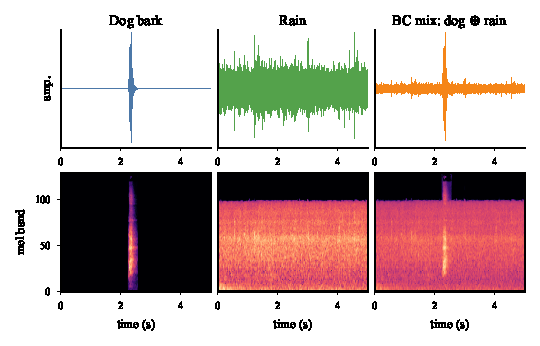
\includegraphics[width=\columnwidth]{fig_dataset.pdf}}
\caption{Raw waveforms (top) and the 128-band log-mel spectrograms FRESCA-Net consumes (bottom) for a dog bark, rain, and their energy-domain Between-Class mixture, computed on the waveform exactly as in training. The mixture preserves total energy: this is the signal the network learns to disentangle.}
\label{fig:data}
\end{figure}

We are explicit about the evaluation being leakage-free, since the small folds make it easy to be optimistic. No early stopping, checkpoint selection or exponential-moving-average selection is ever performed on the test fold. Instead the training budget is fixed in advance at 200 epochs, and the headline number is the stochastic-weight-averaged model \cite{izmailov_swa} formed from the last thirty epochs, with its batch-normalisation statistics recomputed on the training folds only. At inference we average the softmax outputs of three evenly spaced crops of the clip, a label-free test-time augmentation that is standard for ESC-50. Pretrained transformers that use external corpora are outside this comparison and are cited only for orientation.

\subsection{On-GPU Log-Mel Front-End}
The front-end computes a log-mel spectrogram on the GPU with a 1024-point short-time Fourier transform, a 512-sample hop and 128 mel bands, followed by a logarithm. Each spectrogram is standardised per instance to zero mean and unit variance --- deliberately a per-clip statistic, so no train/test normalisation constant is ever shared and the representation is robust to the energy shift introduced by the mixing below. Because a mel axis is not translation-invariant --- a pattern shifted up in frequency is a different sound, not the same sound moved --- we append a fixed frequency-coordinate channel following the CoordConv idea \cite{liu_coordconv}, so the input is a two-channel image of the standardised log-mel and its coordinate map. The transform is parameter-free, which is what allows the augmentation to act on the raw waveform and still be seen by the network as a normal spectrogram.

\subsection{Waveform Augmentation and Energy-Domain Between-Class Learning}\label{sec:aug}
The strongest regulariser in this regime is a random three-second crop at training time, matched at test time by the three-crop averaging above. On top of it we apply mild waveform perturbations --- a circular time shift, a random gain and additive noise at a controlled signal-to-noise ratio --- and a short-ramped SpecAugment on the spectrogram \cite{park_specaugment}.

The principal data lever is Between-Class learning \cite{tokozume_bc}. Two root-mean-square-normalised waveforms $x_1$ and $x_2$ are mixed with a per-sample ratio $p$ drawn uniformly, and the target becomes the same convex combination of their one-hot labels,
\begin{equation}
x = \frac{p\,x_1 + (1-p)\,x_2}{\sqrt{p^2 + (1-p)^2}}, \label{eq:bc}
\end{equation}
where the denominator preserves the energy of the mixture. This is performed on the raw waveform, before the short-time Fourier transform, because sound energy is additive in the waveform domain; mixing already-computed log-mel images would break that energy-additive semantics and change what the ratio means. Between-Class learning is related to the more general mixup \cite{zhang_mixup} but specialised to the physics of the acoustic signal. Label smoothing \cite{muller_labelsmoothing} is applied only on batches where mixing is off, so the two never compound.

\subsection{The FRESCA-Net Architecture}
FRESCA-Net --- for \emph{Frequency-aware Residual Squeeze-Excitation with energy-aware between-Class and Attentive pooling} --- is a squeeze-and-excitation residual network built for the small-data, single-GPU regime. The backbone is an eighteen-layer residual network in the sense of \cite{he_resnet}, with every basic block recalibrated by a squeeze-and-excitation channel-attention unit \cite{hu_senet} and regularised on its residual branch by stochastic depth \cite{huang_stochastic}. Two design choices adapt the generic backbone to spectrograms. First, the downsampling is anisotropic: after an initial isotropic reduction the two deeper stages stride only along frequency, collapsing the frequency axis by a factor of sixteen while dividing the time axis by only four, so that a genuine temporal sequence of about sixty-five frames survives to the top of the network. Second, that sequence is summarised not by a global average but by an attentive-statistics pooling head \cite{okabe_asp}, which learns a per-frame attention weight and returns the attention-weighted mean and standard deviation over time, preserving the temporal salience global pooling discards --- which matters for transients such as a glass break or a dog bark. The complementary idea of factorising a block into a frequency path and a broadcast temporal path \cite{kim_bcresnet} informed the anisotropic design. Fig.~\ref{fig:arch} details the architecture and the tensor shape after every stage at the three-second crop; the network holds 2.88 million trainable parameters. As a controlled baseline we retrain the classic Piczak network \cite{piczak_cnn} under the identical pipeline; its published 64.5 percent is a familiar anchor.

\begin{figure*}[t]
\centerline{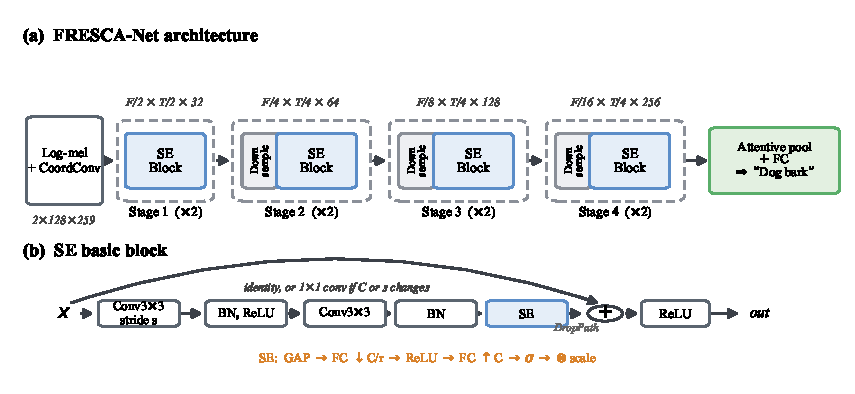
\includegraphics[width=0.72\textwidth]{fig_arch.pdf}}
\caption{FRESCA-Net architecture. (a) A standardised log-mel spectrogram with an appended CoordConv frequency channel enters a stem and four stages of two SE basic blocks each; the two deepest stages stride only along frequency, so $F$ is divided by sixteen while $T$ is divided by only four and a real temporal sequence survives to the attentive-statistics pooling head. (b) One SE basic block: two $3\times3$ convolutions, squeeze-excitation recalibration, and a stochastic-depth residual added to an identity (or $1\times1$-conv) shortcut.}
\label{fig:arch}
\end{figure*}

\subsection{Training Protocol}
Every model is trained end-to-end with the AdamW optimiser \cite{loshchilov_adamw} at a $1\times10^{-3}$ learning rate and $5\times10^{-4}$ weight decay, with batch normalisation and bias parameters excluded from decay. The schedule is a five-epoch linear warm-up followed by cosine annealing \cite{loshchilov_sgdr} down to $1\times10^{-5}$, over the fixed 200-epoch budget, with a batch size of 64 and mixed-precision training on a single CUDA GPU; batch normalisation \cite{ioffe_bn} stabilises the deeper stages. The last thirty epochs feed the stochastic weight average \cite{izmailov_swa} that forms the reported model. This recipe is applied unchanged to every architecture, ablation cell and dataset, so differences in the tables are attributable to the factor under study rather than to per-model tuning; the cost is that no single model is shown at its own optimum. To probe the ceiling of the regime we additionally train a three-seed ensemble: for each held-out fold, three FRESCA-Net models with different seeds are trained on the other four folds for a longer 300-epoch budget and their multi-crop softmax outputs averaged. Every member still sees only folds different from the tested one, so the ensemble remains a leakage-free estimate.

\section{Results and Discussion}

\subsection{Benchmark in Context}
Table~\ref{tab:bench} places FRESCA-Net among the published methods that, like ours, are trained from scratch on ESC-50 without external data. A single FRESCA-Net reaches 81.55 percent, exceeding the crowdsourced human accuracy of 81.3 percent \cite{piczak_dataset} and matching EnvNet-v2 with Between-Class learning at 81.8 percent \cite{tokozume_bc} from only 2.88 million parameters; the three-seed ensemble reaches 82.45 percent, closing much of the remaining gap to the from-scratch state of the art at 84.9 percent \cite{tokozume_bc}. Against the classic anchors the margin is large --- more than seventeen points above the Piczak baseline \cite{piczak_cnn}, and far above the multi-scale \cite{zhu_multiscale} and raw-waveform \cite{tokozume_envnet} entries. Pretrained transformers reaching ninety-five to ninety-eight percent consume the external AudioSet corpus \cite{gemmeke_audioset} and answer a different question.

\begin{table}[t]
\caption{ESC-50 five-fold accuracy in context, from-scratch family (trained on ESC-50 only, no external data). Bold rows are this work.}
\label{tab:bench}
\begin{center}
\renewcommand{\arraystretch}{1.05}
\begin{tabular}{|l|c|}
\hline
\textbf{Method (from scratch)} & \textbf{Acc. (\%)} \\
\hline
EnvNet-v2 $+$ aug $+$ BC learning \cite{tokozume_bc} & 84.90 \\
\textbf{FRESCA-Net, 3-seed ensemble (ours)} & \textbf{82.45} \\
EnvNet-v2 $+$ BC learning \cite{tokozume_bc} & 81.80 \\
\textbf{FRESCA-Net, single model (ours)} & \textbf{81.55} \\
Human accuracy \cite{piczak_dataset} & 81.30 \\
Multi-scale CNN \cite{zhu_multiscale} & 79.10 \\
EnvNet-v2 raw waveform \cite{tokozume_envnet} & 74.40 \\
Piczak CNN \cite{piczak_cnn} & 64.50 \\
Random forest, MFCC $+$ ZCR \cite{piczak_dataset} & 44.30 \\
\hline
\multicolumn{2}{l}{\footnotesize Pretrained transformers reach 95--98\% using external} \\
\multicolumn{2}{l}{\footnotesize data \cite{kong_panns,gong_ast,chen_beats,elizalde_clap} and are out of scope for the from-scratch setting.} \\
\end{tabular}
\end{center}
\end{table}

\subsection{Cost on an Edge Budget}
A parameter count alone does not establish that a model is deployable, so Table~\ref{tab:edge} reports what FRESCA-Net costs at inference: multiply--accumulate operations (MACs) counted analytically per layer and cross-checked against an independent profiler to within 0.8 percent, the fp32 weight footprint and peak batch-of-one activation, and the median of sixty timed runs on one core of an Intel Core i7-12700H, otherwise idle. No microcontroller or single-board computer was available to us, so the MAC and memory columns are device-independent while the latency column characterises one mid-range CPU core, not a specific edge board.

Three observations follow. First, the anisotropic downsampling on which the architecture rests is also its dominant cost: stages three and four, which stride only along frequency and therefore convolve over a sixty-five-frame sequence instead of a sixteen-frame one, account for 1.64 of the 2.23 GMAC, or 73 percent. The choice that buys temporal resolution is the one paid for in arithmetic. Second, MACs are a poor proxy for latency here: FRESCA-Net performs 3.7 times the multiply--accumulates of the Piczak baseline yet is only four percent slower on one core, because Piczak's tall $57\times6$ first-layer filter is memory-bound on a large intermediate activation while FRESCA-Net's $3\times3$ stack is compute-bound and cache-friendly. A 3.7-fold gap in arithmetic that becomes a 1.04-fold gap in time warns that either number alone would mislead. Third, the parameter-free front-end costs 22.9 MMAC per crop, invisible to a parameter count; 17.0 MMAC of that is the dense mel projection, which the 99.5 percent sparsity of the filterbank reduces to 0.26 MMAC. Under the three-crop protocol a five-second clip therefore costs 6.77 GMAC and about 0.31 s on one core, a real-time factor near 0.06, and single-crop inference halves both. Static int8 quantisation compresses the weights from 11.0 to 2.8 MB but gave no latency benefit on this AVX2 host, so we report fp32. A 45 MB peak activation places FRESCA-Net comfortably inside a single-board computer such as a Raspberry Pi but far outside the few hundred kilobytes of SRAM of a microcontroller; we scope our efficiency claim to the former and make none about the latter.

\begin{table}[t]
\caption{Measured inference cost, batch size one, one 3\,s crop. MACs and memory are device-independent; latency is the median of 60 single-thread runs on an Intel Core i7-12700H.}
\label{tab:edge}
\begin{center}
\renewcommand{\arraystretch}{1.05}
\setlength{\tabcolsep}{4pt}
\begin{tabular}{|l|c|c|c|c|c|}
\hline
\textbf{Model} & \textbf{Param} & \textbf{MACs} & \textbf{Weights} & \textbf{Act.} & \textbf{CPU} \\
 & (M) & (G) & (MB) & (MB) & (ms) \\
\hline
\textbf{FRESCA-Net} & 2.88 & 2.23 & 11.0 & 45.2 & 100.1 \\
Piczak CNN & 0.71 & 0.61 & 2.7 & 9.7 & 96.3 \\
\hline
\multicolumn{6}{l}{\footnotesize Log-mel front-end adds 22.9 MMAC and 3.0 ms; three-crop inference of} \\
\multicolumn{6}{l}{\footnotesize a 5\,s clip costs 6.77 GMAC. FRESCA-Net on GPU: 9.3 ms.} \\
\end{tabular}
\end{center}
\end{table}

\subsection{Generalisation to a Second Dataset}
Because a single benchmark cannot separate a good architecture from one fitted to its idiosyncrasies, we retrain FRESCA-Net on UrbanSound8K under its official ten-fold cross-validation, changing only the label space and the fold list. With the epoch budget reduced to 100 and the weight average taken over the last fifteen epochs --- the same fifteen percent tail of the cosine schedule as before, fixed in advance rather than tuned --- it reaches $74.57 \pm 6.10$ percent. That clears the Piczak CNN (73.0) \cite{piczak_cnn}, the unaugmented SB-CNN (74.0) \cite{salamon_bello} and plain EnvNet-v2 (69.1) \cite{tokozume_bc}, but falls short of EnvNet-v2 with Between-Class learning (76.6) and the augmented SB-CNN (79.0). The recipe transfers; the ESC-50 standing does not --- a design that ranks second in the from-scratch family there sits mid-table here.

Two features are worth recording. Our leakage-free rule is dearer here: the averaged model lands 1.91 points \emph{below} the oracle best epoch (76.48), where on ESC-50 it landed 1.35 above, so a protocol selecting epochs on the test fold would report about 76.5 for these runs --- the comparison above is if anything conservative towards us. And the fold spread is more than twice ESC-50's ($\pm6.10$ against $\pm2.83$, from 64.32 to 83.65), consistent with folds drawn from distinct field recordings rather than a balanced pool. The experiment supports the narrow claim that was in doubt --- the architecture is not an artefact of ESC-50's folds --- not the broader one that it is competitive everywhere.

\subsection{Ablation: Architecture, Augmentation and Weight Averaging}
To separate the contribution of the network from that of the augmentation we run the two-by-two matrix of Table~\ref{tab:ablation}, in which FRESCA-Net and the Piczak baseline are each trained with the full augmentation pipeline and with none, under the identical protocol and seed. Replacing the Piczak baseline with FRESCA-Net, at no augmentation, adds 16.45 points (62.20 to 78.65 percent); adding the full augmentation to FRESCA-Net adds a further 2.90 points (78.65 to 81.55 percent). For this compact-but-strong backbone the architecture is by far the dominant lever and the augmentation a useful but secondary refinement. The Piczak baseline behaves oppositely --- augmentation moves it 8.05 points (62.20 to 70.25 percent) --- because a weaker network leaves more of the accuracy for the data pipeline to recover. A capable backbone therefore internalises much of what augmentation must otherwise supply.

The same table isolates the cost of our leakage-free rule. For the full FRESCA-Net pipeline the averaged model scores 81.55 percent, 4.45 points above the last-epoch model and 1.35 points above even the single best epoch --- and that best epoch is an oracle, identifiable only by peeking at the fold being tested. Weight averaging therefore does more than remove the temptation to select on the test fold: it beats what such selection could have achieved, so we fix the epoch budget in advance without paying an accuracy penalty for honesty. The benefit is specific to the augmented regime: without augmentation the trajectory is smooth, the last-epoch and averaged models coincide (78.75 against 78.65 percent), and the weak Piczak baseline behaves the same way. It is only when Between-Class and SpecAugment noise makes the late iterates a poor summary of a wide optimum that averaging the last thirty epochs recovers a markedly better solution.

\begin{table}[t]
\caption{Matched ablation and weight averaging under one protocol and seed. Mean five-fold accuracy (\%) of the last-epoch model, the single best epoch, and the reported SWA model ($\pm$ standard deviation across folds).}
\label{tab:ablation}
\begin{center}
\renewcommand{\arraystretch}{1.05}
\begin{tabular}{|l|c|c|c|}
\hline
\textbf{Configuration} & \textbf{Last} & \textbf{Best$^{\mathrm{a}}$} & \textbf{SWA (reported)} \\
\hline
\textbf{FRESCA-Net}, full aug & 77.10 & 80.20 & $\mathbf{81.55 \pm 2.83}$ \\
FRESCA-Net, no aug & 78.75 & 79.90 & $78.65 \pm 3.39$ \\
Piczak CNN, full aug & 70.10 & 71.45 & $70.25 \pm 1.39$ \\
Piczak CNN, no aug & 62.20 & 63.90 & $62.20 \pm 4.11$ \\
\hline
\multicolumn{4}{l}{\footnotesize $^{\mathrm{a}}$Best epoch requires selecting on the test fold (leaky); listed} \\
\multicolumn{4}{l}{\footnotesize only to show that SWA does not sacrifice accuracy. Architecture} \\
\multicolumn{4}{l}{\footnotesize at no aug: $+16.45$ pt; augmentation on FRESCA-Net: $+2.90$ pt,} \\
\multicolumn{4}{l}{\footnotesize on Piczak: $+8.05$ pt. FRESCA-Net 2.88\,M vs Piczak 0.71\,M param.} \\
\end{tabular}
\end{center}
\end{table}

\subsection{Per-Fold Behaviour and the Ensemble}
Figure~\ref{fig:folds} shows the single model and the three-seed ensemble on each of the five folds. The single model swings from 77.50 to 85.75 percent, a spread symptomatic of the sixteen-hundred-clip regime rather than of the model. The ensemble is steadier: it lifts the two weakest folds while barely changing the strongest, so the standard deviation falls from 2.83 to 1.60 points and the mean rises to 82.45 percent. The gain is not simply more compute: the three seeds, trained for the longer 300-epoch budget, individually average only 79.92 percent --- below the 200-epoch single model, confirming that the extra epochs overfit --- yet averaging them yields a 2.53-point gain, largest where the seeds disagree most ($+3.50$ on the weakest fold five, $+3.25$ on fold one). A dataset-level regularity is also visible: fold four is the easiest in four of the five configurations of Table~\ref{tab:ablation} and for the ensemble, and fold five the hardest in four of five, a pattern that largely survives changes of architecture and so reflects how the official folds partition the classes rather than any instability of the model. The exception is the weakest configuration, the unaugmented Piczak baseline, whose fold ordering is least stable.

\begin{figure}[t]
\centerline{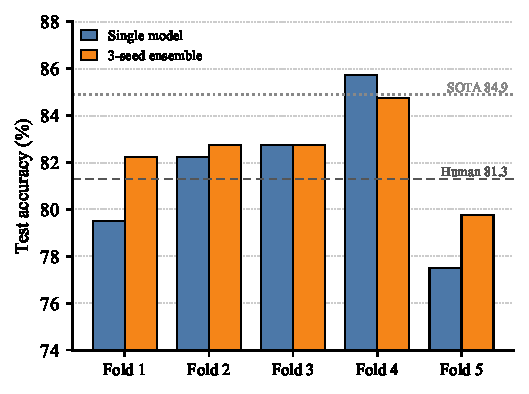
\includegraphics[width=0.62\columnwidth]{fig_folds.pdf}}
\caption{Per-fold accuracy of the single FRESCA-Net (200 epochs, three-crop TTA) and the three-seed ensemble (300 epochs, seven-crop). Reference lines: human accuracy (81.3) and from-scratch state of the art (84.9).}
\label{fig:folds}
\end{figure}

\subsection{Discussion and Limitations}
Four observations stand out. First, on a small, hard, from-scratch benchmark the architecture is the primary determinant of accuracy: the compact residual backbone with channel attention and a temporal-aware pooling head buys sixteen points over the classic baseline before any augmentation, whereas augmentation adds under three. Modern design choices matter chiefly by making a small network optimise stably from little data rather than by adding representational power. Second, among the augmentations it is the energy-domain Between-Class mixing, applied in the waveform domain so that its energy-additive semantics stay exact, that keeps paying on top of a strong backbone \cite{tokozume_bc}. Third, the bottleneck is the data, not the capacity: the 300-epoch over-training result and the fold-to-fold variance both point to the sixteen-hundred-clip regime as the ceiling. Fourth, efficiency claims need measuring rather than asserting --- on our own model the parameter count, the MAC count and the measured latency each tell a different story.

Limitations remain. The study is confined by design to the from-scratch setting, so pretrained transformers are cited only for orientation, and a single shared recipe isolates each factor at one fixed cost without showing any model at its own optimum. The costs in Table~\ref{tab:edge} come from a desktop-class CPU core rather than an edge board: they bound arithmetic and memory exactly but only indicate the latency such a board would see. The UrbanSound8K run uses a reduced budget and one seed, so its absolute figure is a lower bound rather than this architecture's best; a per-class confusion study across seeds remains future work.

\subsection{Reproducibility and Availability}
Both benchmarks are public: ESC-50 \cite{piczak_dataset} and UrbanSound8K \cite{salamon_urbansound} are distributed by their authors with the fold assignments we use unmodified, and no other data enters training. To let the protocol be checked rather than taken on trust, we release the complete implementation --- front-end, Between-Class mixing, both architectures, the fold-wise trainer, the cost profiler, and the exact commands, seeds and per-fold results behind every number here --- at \texttt{https://github.com/SeedFlora/fresca}.

\section{Conclusion}
We presented FRESCA-Net, a compact 2.88 million-parameter convolutional network trained entirely from scratch on ESC-50 and evaluated under a single leakage-free five-fold protocol. Its frequency-aware squeeze-and-excitation backbone, anisotropic downsampling, attentive-statistics pooling and energy-domain Between-Class augmentation reach 81.55 percent as a single model and 82.45 percent as a three-seed ensemble, exceeding human accuracy and matching EnvNet-v2 with Between-Class learning without any external data. A matched ablation attributes the bulk of the accuracy to the architecture ($+16.45$ points) over the augmentation ($+2.90$), and the per-fold study exposes the small-data regime, not model capacity, as the ceiling. Carried over unchanged to UrbanSound8K it reaches 74.57 percent --- above the classic from-scratch baselines but below the augmented ones, so the architecture transfers while its ESC-50 ranking does not --- and a direct measurement of arithmetic, memory and latency locates the model on a single-board computer rather than a microcontroller while showing that MAC counts alone would have ranked it wrongly. The work offers a reproducible reference for compact, from-scratch environmental sound recognition and a clean protocol on which future data-centric gains can be measured.

\begin{thebibliography}{00}
\bibitem{piczak_dataset} K. J. Piczak, ``ESC: Dataset for environmental sound classification,'' in \textit{Proc. ACM Int. Conf. Multimedia (MM)}, 2015, pp. 1015--1018, doi: 10.1145/2733373.2806390.
\bibitem{salamon_urbansound} J. Salamon, C. Jacoby, and J. P. Bello, ``A dataset and taxonomy for urban sound research,'' in \textit{Proc. ACM Int. Conf. Multimedia (MM)}, 2014, pp. 1041--1044, doi: 10.1145/2647868.2655045.
\bibitem{piczak_cnn} K. J. Piczak, ``Environmental sound classification with convolutional neural networks,'' in \textit{Proc. IEEE Int. Workshop Mach. Learn. Signal Process. (MLSP)}, 2015, pp. 1--6, doi: 10.1109/MLSP.2015.7324337.
\bibitem{salamon_bello} J. Salamon and J. P. Bello, ``Deep convolutional neural networks and data augmentation for environmental sound classification,'' \textit{IEEE Signal Process. Lett.}, vol. 24, no. 3, pp. 279--283, 2017, doi: 10.1109/LSP.2017.2657381.
\bibitem{tokozume_envnet} Y. Tokozume and T. Harada, ``Learning environmental sounds with end-to-end convolutional neural network,'' in \textit{Proc. IEEE ICASSP}, 2017, pp. 2721--2725, doi: 10.1109/ICASSP.2017.7952651.
\bibitem{dai_rawwaveform} W. Dai, C. Dai, S. Qu, J. Li, and S. Das, ``Very deep convolutional neural networks for raw waveforms,'' in \textit{Proc. IEEE ICASSP}, 2017, pp. 421--425, doi: 10.1109/ICASSP.2017.7952190.
\bibitem{huzaifah_tf} M. Huzaifah, ``Comparison of time-frequency representations for environmental sound classification using convolutional neural networks,'' arXiv:1706.07156, 2017.
\bibitem{tokozume_bc} Y. Tokozume, Y. Ushiku, and T. Harada, ``Learning from between-class examples for deep sound recognition,'' in \textit{Proc. ICLR}, 2018, arXiv:1711.10282.
\bibitem{zhu_multiscale} B. Zhu, C. Wang, F. Liu, J. Lei, Z. Lu, and Y. Peng, ``Learning environmental sounds with multi-scale convolutional neural network,'' in \textit{Proc. IJCNN}, 2018, pp. 1--8, doi: 10.1109/IJCNN.2018.8489641.
\bibitem{aytar_soundnet} Y. Aytar, C. Vondrick, and A. Torralba, ``SoundNet: Learning sound representations from unlabeled video,'' in \textit{Proc. NeurIPS}, vol. 29, 2016, pp. 892--900.
\bibitem{hershey_cnnaudio} S. Hershey \textit{et al.}, ``CNN architectures for large-scale audio classification,'' in \textit{Proc. IEEE ICASSP}, 2017, pp. 131--135, doi: 10.1109/ICASSP.2017.7952132.
\bibitem{gemmeke_audioset} J. F. Gemmeke \textit{et al.}, ``Audio Set: An ontology and human-labeled dataset for audio events,'' in \textit{Proc. IEEE ICASSP}, 2017, pp. 776--780, doi: 10.1109/ICASSP.2017.7952261.
\bibitem{kong_panns} Q. Kong, Y. Cao, T. Iqbal, Y. Wang, W. Wang, and M. D. Plumbley, ``PANNs: Large-scale pretrained audio neural networks for audio pattern recognition,'' \textit{IEEE/ACM Trans. Audio, Speech, Language Process.}, vol. 28, pp. 2880--2894, 2020, doi: 10.1109/TASLP.2020.3030497.
\bibitem{gong_ast} Y. Gong, Y.-A. Chung, and J. Glass, ``AST: Audio spectrogram transformer,'' in \textit{Proc. Interspeech}, 2021, pp. 571--575, doi: 10.21437/Interspeech.2021-698.
\bibitem{chen_beats} S. Chen \textit{et al.}, ``BEATs: Audio pre-training with acoustic tokenizers,'' in \textit{Proc. ICML}, PMLR vol. 202, 2023, pp. 5178--5193.
\bibitem{elizalde_clap} B. Elizalde, S. Deshmukh, M. Al Ismail, and H. Wang, ``CLAP: Learning audio concepts from natural language supervision,'' in \textit{Proc. IEEE ICASSP}, 2023, doi: 10.1109/ICASSP49357.2023.10095889.
\bibitem{guzhov_esresnet} A. Guzhov, F. Raue, J. Hees, and A. Dengel, ``ESResNet: Environmental sound classification based on visual domain models,'' in \textit{Proc. ICPR}, 2021, pp. 4933--4940, doi: 10.1109/ICPR48806.2021.9413035.
\bibitem{palanisamy_rethinking} K. Palanisamy, D. Singhania, and A. Yao, ``Rethinking CNN models for audio classification,'' arXiv:2007.11154, 2020.
\bibitem{izmailov_swa} P. Izmailov, D. Podoprikhin, T. Garipov, D. Vetrov, and A. G. Wilson, ``Averaging weights leads to wider optima and better generalization,'' in \textit{Proc. UAI}, 2018, pp. 876--885.
\bibitem{liu_coordconv} R. Liu \textit{et al.}, ``An intriguing failing of convolutional neural networks and the CoordConv solution,'' in \textit{Proc. NeurIPS}, 2018, pp. 9628--9639.
\bibitem{park_specaugment} D. S. Park \textit{et al.}, ``SpecAugment: A simple data augmentation method for automatic speech recognition,'' in \textit{Proc. Interspeech}, 2019, pp. 2613--2617, doi: 10.21437/Interspeech.2019-2680.
\bibitem{zhang_mixup} H. Zhang, M. Cisse, Y. N. Dauphin, and D. Lopez-Paz, ``mixup: Beyond empirical risk minimization,'' in \textit{Proc. ICLR}, 2018, arXiv:1710.09412.
\bibitem{muller_labelsmoothing} R. M\"uller, S. Kornblith, and G. E. Hinton, ``When does label smoothing help?,'' in \textit{Proc. NeurIPS}, 2019, pp. 4694--4703.
\bibitem{he_resnet} K. He, X. Zhang, S. Ren, and J. Sun, ``Deep residual learning for image recognition,'' in \textit{Proc. IEEE CVPR}, 2016, pp. 770--778, doi: 10.1109/CVPR.2016.90.
\bibitem{hu_senet} J. Hu, L. Shen, and G. Sun, ``Squeeze-and-excitation networks,'' in \textit{Proc. IEEE CVPR}, 2018, pp. 7132--7141, doi: 10.1109/CVPR.2018.00745.
\bibitem{huang_stochastic} G. Huang, Y. Sun, Z. Liu, D. Sedra, and K. Q. Weinberger, ``Deep networks with stochastic depth,'' in \textit{Proc. ECCV}, 2016, pp. 646--661, doi: 10.1007/978-3-319-46493-0\_39.
\bibitem{okabe_asp} K. Okabe, T. Koshinaka, and K. Shinoda, ``Attentive statistics pooling for deep speaker embedding,'' in \textit{Proc. Interspeech}, 2018, pp. 2252--2256, doi: 10.21437/Interspeech.2018-993.
\bibitem{kim_bcresnet} B. Kim, S. Chang, J. Lee, and D. Sung, ``Broadcasted residual learning for efficient keyword spotting,'' in \textit{Proc. Interspeech}, 2021, pp. 4538--4542, doi: 10.21437/Interspeech.2021-383.
\bibitem{loshchilov_adamw} I. Loshchilov and F. Hutter, ``Decoupled weight decay regularization,'' in \textit{Proc. ICLR}, 2019, arXiv:1711.05101.
\bibitem{loshchilov_sgdr} I. Loshchilov and F. Hutter, ``SGDR: Stochastic gradient descent with warm restarts,'' in \textit{Proc. ICLR}, 2017, arXiv:1608.03983.
\bibitem{ioffe_bn} S. Ioffe and C. Szegedy, ``Batch normalization: accelerating deep network training by reducing internal covariate shift,'' in \textit{Proc. ICML}, PMLR vol. 37, 2015, pp. 448--456.
\end{thebibliography}

\end{document}
